\documentclass{article}
\usepackage[utf8]{inputenc}
\usepackage[margin=0.35in]{geometry}
\usepackage{natbib}
\usepackage{graphicx}

\title{CPEG 457 Assignment 2}
\author{Shane Cincotta }
\date{April 6, 2020}

\begin{document}
\maketitle

\section*{Part 1}
\subsection*{1}
\begin{figure}[h!]
\centering
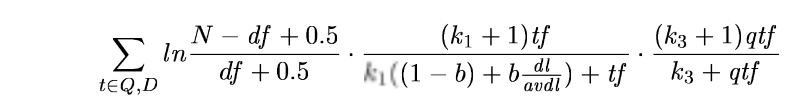
\includegraphics[scale=0.35]{Okapi_FORMULA_MATH.png}
\caption{Okapi Mathematical Formula}
\end{figure}

\begin{figure}[h!]
\centering
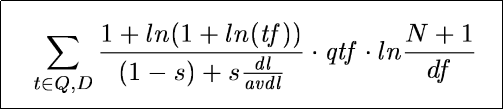
\includegraphics[scale=0.35]{TF_IDF_FORMULA_MATH.png}
\caption{TF-IDF Mathematical Formula}
\end{figure}

Both of the formulas for the Oakpi and TF-IDF retrieval methods incorporate the total number of documents in the collection, the term's frequency in the document, the terms frequency in the query, the number of documents that contain the term, the document length and the average document length.  Also, both formulas use $C*\frac{dl}{avdl}$ in the denominator, where $C$ is a constant, $dl$ is the document length and $avdl$ is the average document length.\\
\newline On the other hand, the formulas also contain unshared terms.  The Okapi formula has 3 distinct contstants, $k_1$, $k_3$ and $b$, while the TF-IDF formula has 1 distinc constant, $s$.\\
\subsection*{2}

\begin{figure}[h!]
\centering
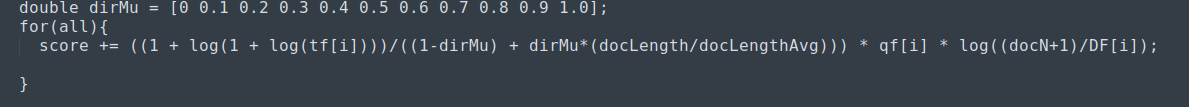
\includegraphics[scale=0.45]{TF_IDF_FORMULA.png}
\caption{TF-IDF Formula}
\end{figure}

Figure 3 shows the implemented TF-IDF formula with the value of $b$ set by the variable dirMu.\\

\begin{figure}[h!]
\centering
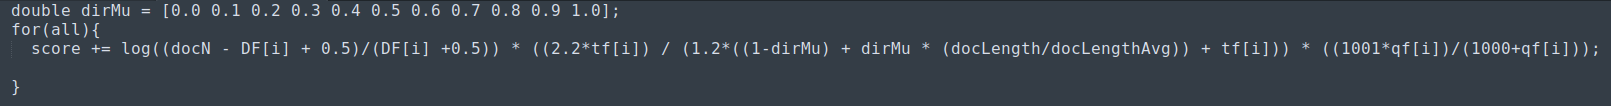
\includegraphics[scale=0.35]{Okapi_FORMULA.png}
\caption{Okapi Formula}
\end{figure}

Figure 4 shows the implemented TF-IDF formula with the value of $s$ set by the variable dirMu.\\

\clearpage

\subsection*{3}
\begin{figure}[h!]
\centering
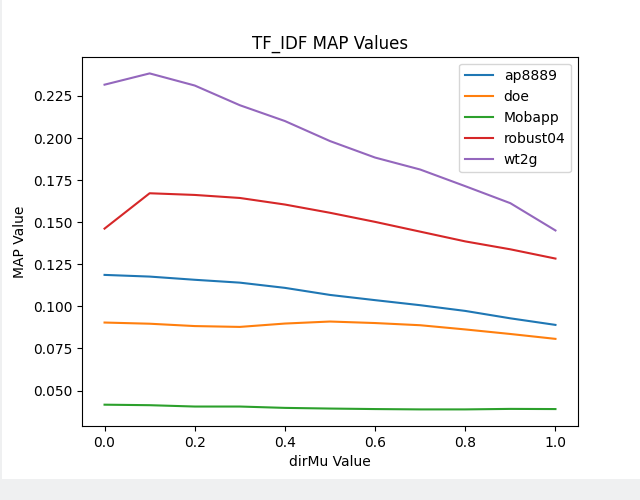
\includegraphics[scale=0.35]{TF_IDF_MAP_VALUES.png}
\caption{TF-IDF Map Values}
\end{figure}

\begin{figure}[h!]
\centering
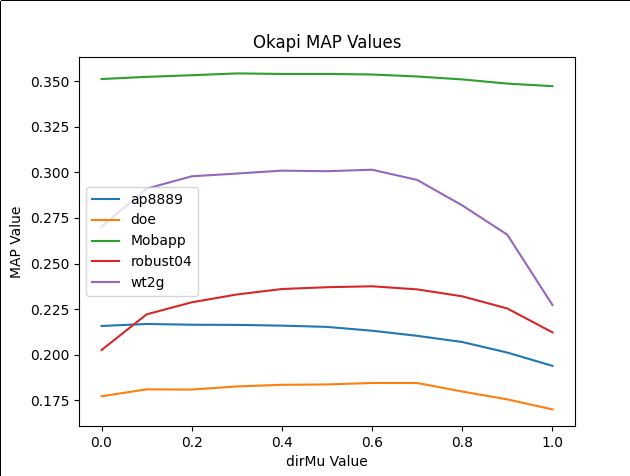
\includegraphics[scale=0.35]{OKAPI_MAP_VALUES.png}
\caption{Okapi Map Values}
\end{figure}

Figures 5 and 6 show the performace of the above retrieval formulas with 11 dirMu values (0-1) tested against 5 collections.\\
\newline According to figures 5 and 6, when optimally tuned, the Okapi formula produced the best results against every collection.\\
\newline Additionally, the formulas do appear to have different sensitivities to the setting of the dirMu parameter.  According to the TF-IDF results, an increase in the dirMu parameter generally correlates with a decrease of the MAP value in a semi-linear fashion.\\
\newline This contrasts with the Okapi results.  According to figure 6, an increase in the dirMu parameter generally correlates with a increase of the MAP value.  This trend continues until dirMu reaches about 0.6, at which point an increase of the dirMu parameter generally results in a decrease of the MAP value.\\
\newline The results also vary widely depending on the collection used.  For example, the Okapi formula has a roughly steady MAP value of 0.35 when tested with the Mobapp collection.  But the formula has a roughly steady MAP value of 0.18 when tested with the doe collection, around a 50 percent decrease.  Another interesting observation is that there does not seem to be a constant rank regarding difficulty of the collections, that is, just because Okapi did poorly with one collection relative to the other collections, does not mean that TF-IDF will also perform poorly.  For example, the Okapi method performed the best with the Mobapp collection, yet the TF-IDF method performed the worst with that same collection.\\
\clearpage

\section*{Part 2}
\subsection*{BM25Plus}
For my first retrieval function, I implemented the BM25Plus method.  Figure 7 shows the mathematical formula, figure 8 shows the formula translated to code and figures 9 and 10 show graphs of the results.\\

\begin{figure}[h!]
\centering
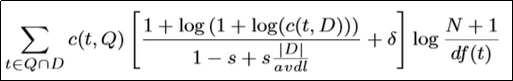
\includegraphics[scale=0.45]{BM25Plus_FORMULA_MATH.png}
\caption{}
\end{figure}

\begin{figure}[h!]
\centering
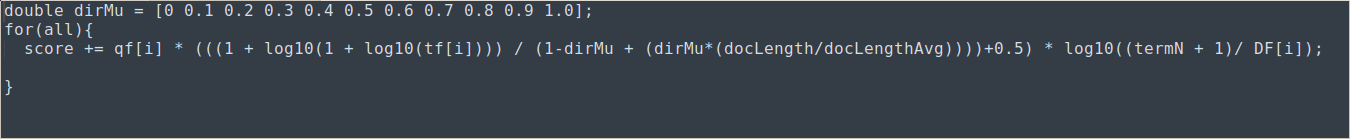
\includegraphics[scale=0.45]{BM25Plus_FORMULA.png}
\caption{}
\end{figure}

\begin{figure}[h!]
\centering
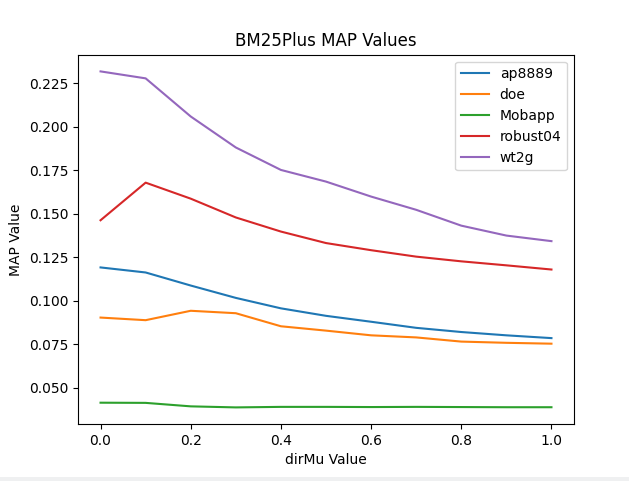
\includegraphics[scale=0.40]{BM25Plus_MAP_VALUES.png}
\caption{}
\end{figure}

\begin{figure}[h!]
\centering
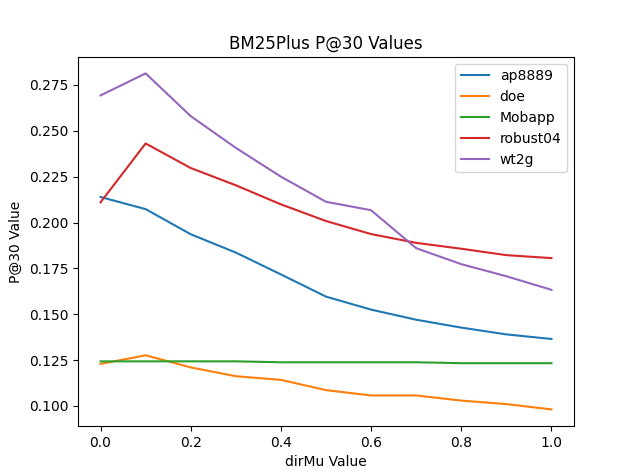
\includegraphics[scale=0.40]{BM25Plus_P30_VALUES.png}
\caption{}
\end{figure}
\clearpage

\subsection*{PL2}
For my second retrieval function, I implemented the PL2 method.  Figures 11 and 12 show the mathematical formula, figure 13 shows the formula translated to code and figures 14 and 15 show graphs of the results.\\

\begin{figure}[h!]
\centering
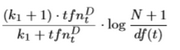
\includegraphics[scale=0.45]{PL2_FORMULA_MATH_1.png}
\caption{}
\end{figure}

\begin{figure}[h!]
\centering
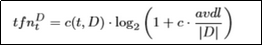
\includegraphics[scale=0.45]{PL2_FORMULA_MATH_2.png}
\caption{}
\end{figure}

\begin{figure}[h!]
\centering
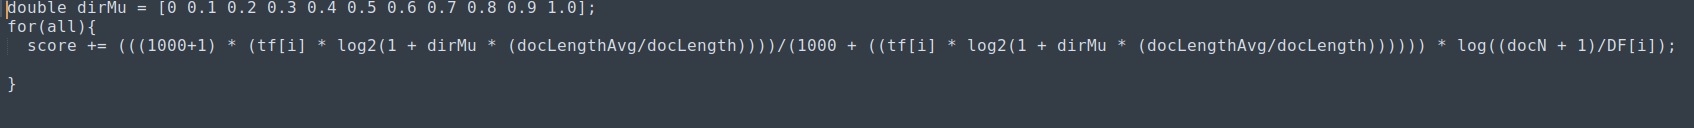
\includegraphics[scale=0.45]{PL2_FORMULA.png}
\caption{}
\end{figure}

\begin{figure}[h!]
\centering
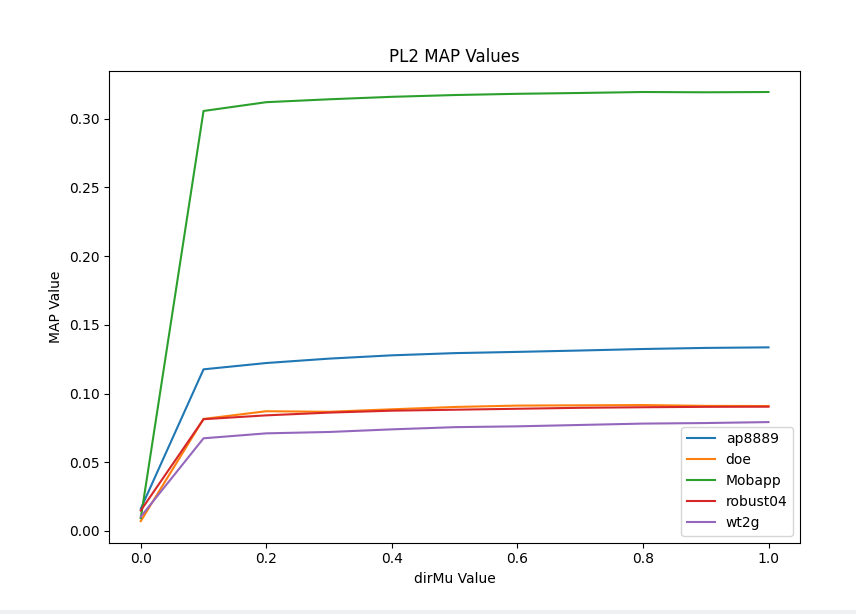
\includegraphics[scale=0.30]{PL2_MAP_VALUES.png}
\caption{}
\end{figure}

\begin{figure}[h!]
\centering
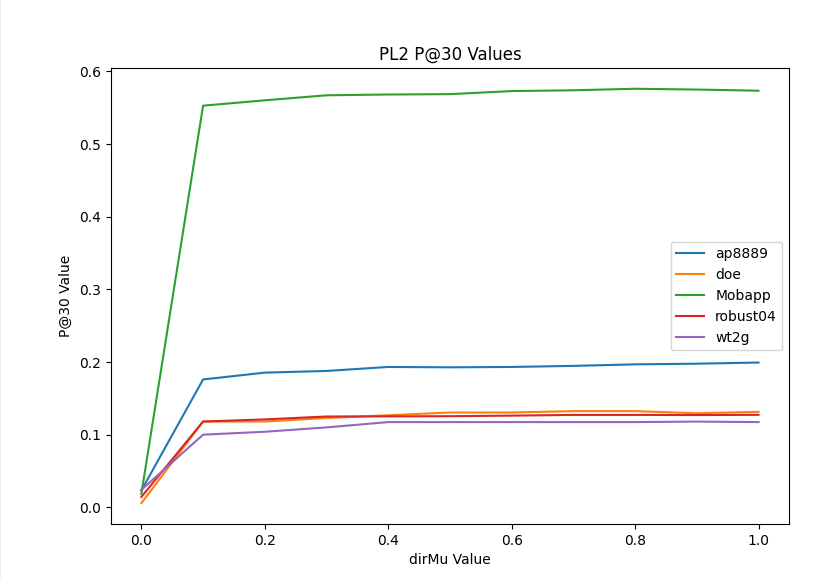
\includegraphics[scale=0.30]{PL2_P30_VALUES.png}
\caption{}
\end{figure}
\clearpage

\subsection*{F1-Log}
For my last retrieval function, I implemented the F1-Log method.  Figure 16 shows the mathematical formula, figure 17 shows the formula translated to code and figures 18 and 19 show graphs of the results.\\

\begin{figure}[h!]
\centering
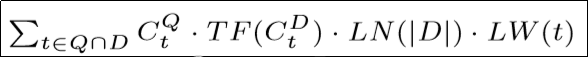
\includegraphics[scale=0.45]{F1_LOG_FORMULA_MATH.png}
\caption{}
\end{figure}

\begin{figure}[h!]
\centering
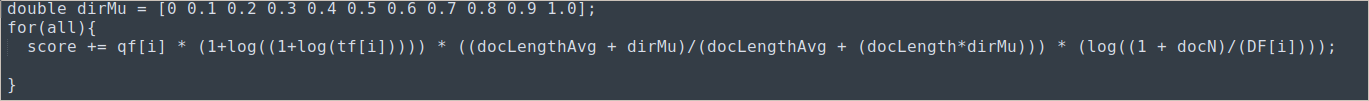
\includegraphics[scale=0.45]{F1_LOG_FORMULA.png}
\caption{}
\end{figure}

\begin{figure}[h!]
\centering
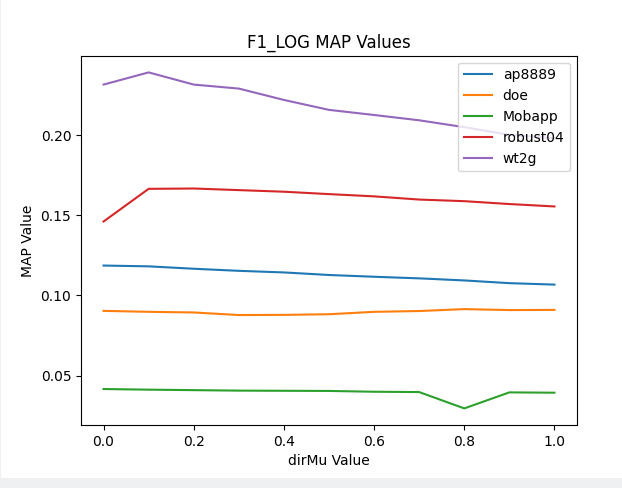
\includegraphics[scale=0.40]{F1_LOG_MAP_VALUES.png}
\caption{}
\end{figure}

\begin{figure}[h!]
\centering
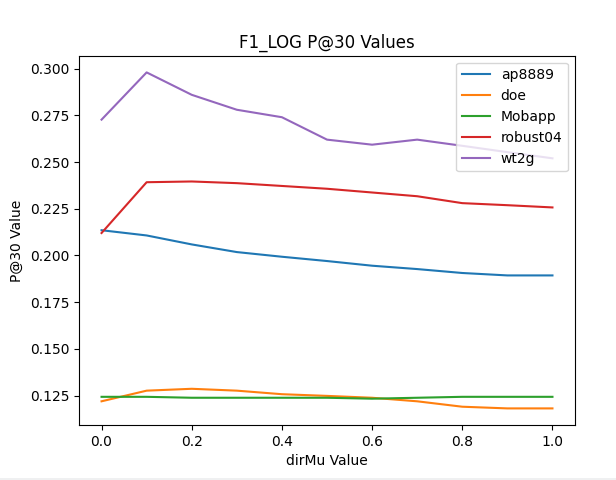
\includegraphics[scale=0.40]{F1_LOG_P30_VALUES.png}
\caption{}
\end{figure}
\end{document}


% \begin{figure}[h!]
% \centering
% 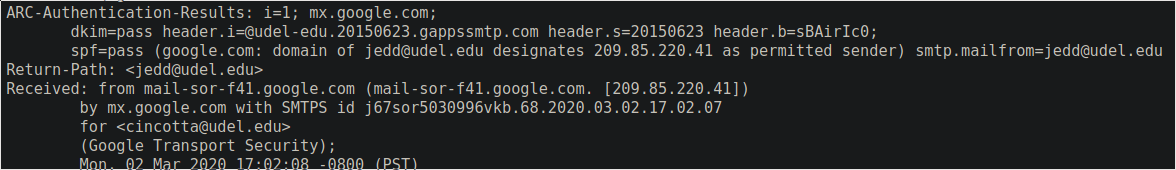
\includegraphics[scale=0.65]{RQ20a.png}
% \caption{}
% \end{figure}

% For each function, please describe the name used in the system, your
% implemented code as well as their mathematic formulas and graph of results